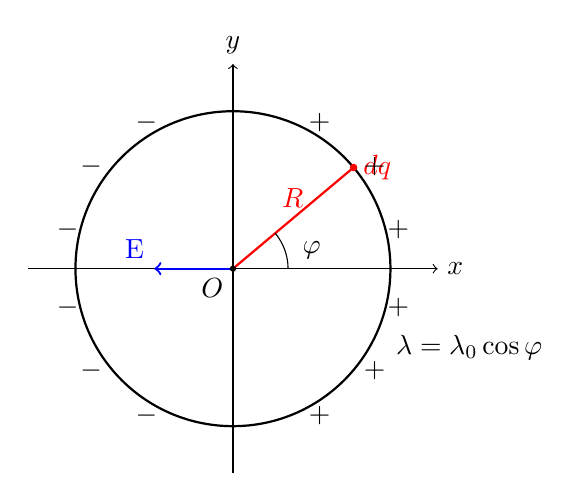
\begin{tikzpicture}[scale=2]

% O'qlar
\draw[->] (-1.3,0) -- (1.3,0) node[right] {$x$};
\draw[->] (0,-1.3) -- (0,1.3) node[above] {$y$};

% Halqa
\draw[thick] (0,0) circle(1);

% Radius
\draw[thick,red] (0,0) -- ({cos(40)},{sin(40)});
\node[red] at (0.38,0.45) {$R$};

% Burchak
\draw (0.35,0) arc(0:40:0.35);
\node at (0.5,0.12) {$\varphi$};

% dq elementi
\filldraw[red] ({cos(40)},{sin(40)}) circle(0.02);
\node[red,right] at ({cos(40)},{sin(40)}) {$dq$};

\draw[thick,->,blue] (0,0)--(-0.5,0) node[above left] {E};
% Markaz
\fill (0,0) circle(0.02);
\node[below left] at (0,0) {$O$};

% Zaryad zichligi yozuvi
\node at (1.5,-0.5) {$\lambda=\lambda_0\cos\varphi$};

% Musbat zaryadlar (o'ng tomon)
\node at (1.05,0.25) {$+$};
\node at (0.9,0.65) {$+$};
\node at (0.55,0.93) {$+$};
\node at (1.05,-0.25) {$+$};
\node at (0.9,-0.65) {$+$};
\node at (0.55,-0.93) {$+$};

% Manfiy zaryadlar (chap tomon)
\node at (-1.05,0.25) {$-$};
\node at (-0.9,0.65) {$-$};
\node at (-0.55,0.93) {$-$};
\node at (-1.05,-0.25) {$-$};
\node at (-0.9,-0.65) {$-$};
\node at (-0.55,-0.93) {$-$};

\end{tikzpicture}


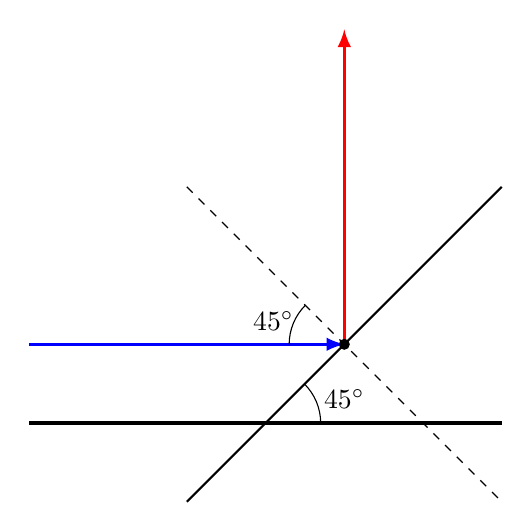
\begin{tikzpicture}[>=latex,scale=1]

% Ko‘zgu
\draw[thick] (-2,-2)--(2,2);

% Normal
\draw[dashed] (-2,2)--(2,-2);

% Tushuvchi nur
\draw[blue,very thick,->] (-4,0)--(0,0);
\draw[very thick] (-4,-1)--(2,-1);

% Qaytgan nur
\draw[red,very thick,->] (0,0)--(0,4);

% Markaz
\fill (0,0) circle(2pt);

% 45 gradus burchaklar
\draw (-0.3,-1) arc[start angle=0,end angle=45,radius=0.7];
\node at (0,-0.7) {$45^\circ$};

\draw (-0.7,0) arc[start angle=180,end angle=135,radius=0.7];
\node at (-0.9,0.3) {$45^\circ$};

\end{tikzpicture}







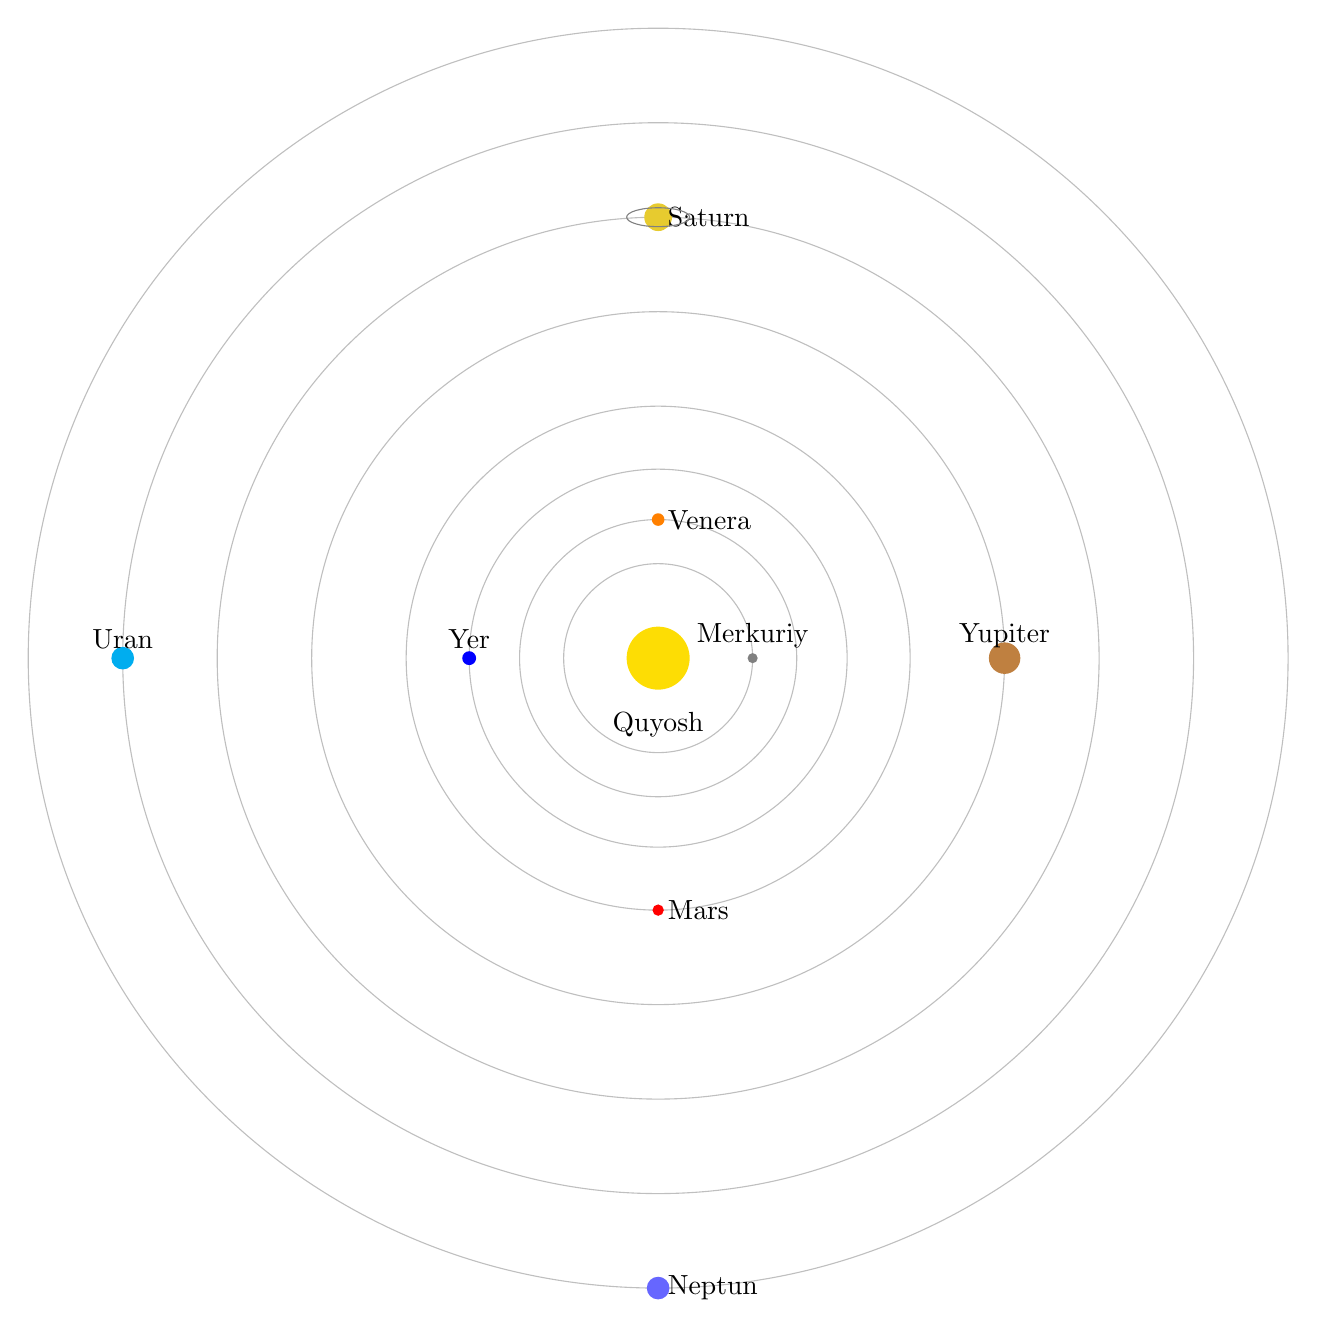
\begin{tikzpicture}[scale=0.8]

% Quyosh
\fill[yellow!80!orange] (0,0) circle (0.5);
\node[below] at (0,-0.7) {Quyosh};

% Orbitlar
\foreach \r in {1.5,2.2,3.0,4.0,5.5,7.0,8.5,10.0}
{
    \draw[gray!50] (0,0) circle (\r);
}

% Sayyoralar
\fill[gray]      (1.5,0) circle (0.08);
\node[above] at (1.5,0) {Merkuriy};

\fill[orange]    (0,2.2) circle (0.10);
\node[right] at (0,2.2) {Venera};

\fill[blue]      (-3.0,0) circle (0.11);
\node[above] at (-3.0,0) {Yer};

\fill[red]       (0,-4.0) circle (0.09);
\node[right] at (0,-4.0) {Mars};

\fill[brown]     (5.5,0) circle (0.25);
\node[above] at (5.5,0) {Yupiter};

\fill[yellow!60!brown] (0,7.0) circle (0.22);
\node[right] at (0,7.0) {Saturn};

% Saturn halqasi
\draw[gray] (0,7.0) ellipse (0.5 and 0.15);

\fill[cyan]      (-8.5,0) circle (0.18);
\node[above] at (-8.5,0) {Uran};

\fill[blue!60]   (0,-10.0) circle (0.18);
\node[right] at (0,-10.0) {Neptun};

\end{tikzpicture}




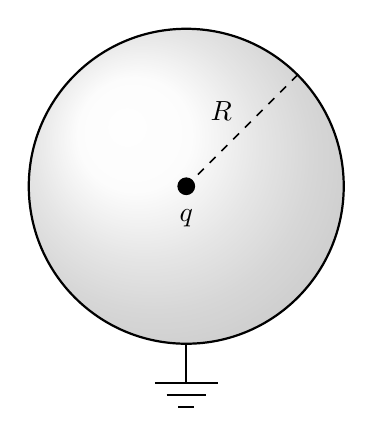
\begin{tikzpicture}
    % Sferaga 3D effekt berish uchun ball shading ishlatamiz
    \shade[ball color = gray!10, opacity=0.3] (0,0) circle (2cm);
    \draw[thick] (0,0) circle (2cm);
    
    % Markazdagi nuqtaviy zaryad
    \filldraw (0,0) circle (3pt) node[below=5pt] {$q$};
    
    % Radius chizig'i - aniqroq ko'rinishi uchun uzuq-uzuq chiziqda
    \draw[dashed, semithick] (0,0) -- (45:2cm) node[midway, above left] {$R$};
    
    % Yerga ulash (Grounding) qismini pastga surish va chizish
    \begin{scope}[shift={(0,-2cm)}]
        \draw[thick] (0,0) -- (0,-0.5);
        \draw[thick] (-0.4,-0.5) -- (0.4,-0.5);
        \draw[thick] (-0.25,-0.65) -- (0.25,-0.65);
        \draw[thick] (-0.1,-0.8) -- (0.1,-0.8);
    \end{scope}
    
\end{tikzpicture}




\begin{tikzpicture}[
    >=Stealth,
    line cap=round,
    line join=round,
    thick,
    font=\large
]

% =========================================================
% PARAMETRLAR
% =========================================================

\def\R{2.35}      % sfera radiusi
\coordinate (O) at (0,0);

% Kirish nuqtasi
\coordinate (P) at (-2.3,0.55);

% Chiqish nuqtasi A
\coordinate (A) at (2.3,0.55);

% =========================================================
% SFERA
% =========================================================

\draw (O) circle (\R);
\draw[dashed] (O) -- (4.6,1.1);
\draw[dashed] (O) -- (-4.6,1.1);

\node[left] at (-2.6,0.5) {$\alpha$};
\node[left] at (-1,0.35) {$\beta$};

\node[left] at (3.2,0.5) {$\alpha$};
\node[left] at (1.2,0.35) {$\beta$};

% Markaz
\fill (O) circle (1.5pt);
\node[below=2pt] at (O) {$O$};

% =========================================================
% TASHQI KIRUVCHI NUR
% =========================================================

\draw[->]
    (-4.0,-0.15) -- (P);
\draw[->]
     (A)--(4.0,-0.15);
% =========================================================
% SFERA ICHIDAGI NUR
% =========================================================

\draw[->]
    (P) -- (A);



% =========================================================
% A NUQTASI
% =========================================================

\fill (A) circle (2pt);

\node[above right=2pt] at (A) {$A$};



\end{tikzpicture}
